%!TEX root = ../Thesis.tex
\chapter{Service Requirements for Aggregators} % (fold)
\label{cha:services}
\begin{marginfigure}
	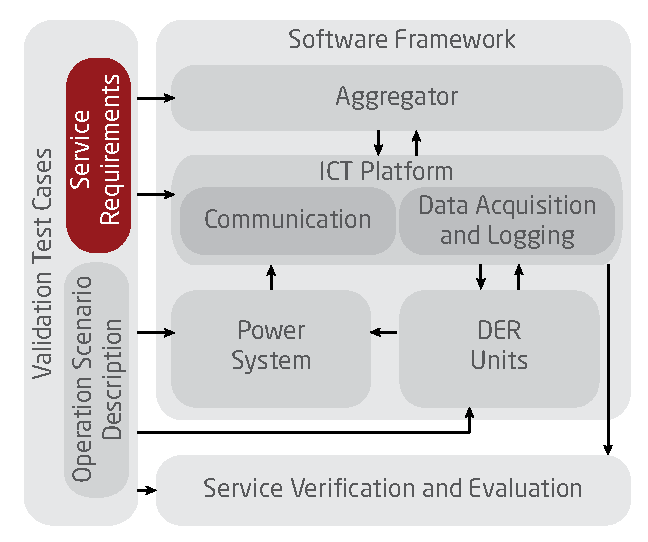
\includegraphics[width=\textwidth]{framework_services.eps}
	\caption{This chapter focuses on the \emph{service definition} block of the aggregator validation framework presented in Chapter~\ref{cha:validation}.}
      \label{fig:framework_services}
\end{marginfigure}
\newchapter{I}{t is clear from} Chapter~\ref{cha:validation} that \emph{service requirements} is an essential block in the aggregator validation framework (see Figure~\ref{fig:framework_services}). Initially, an objective of this work was to model service requirements in order to perform the aggregator validation. While this objective was achieved, it is clear that current service requirements in many countries are directly, or indirectly, blocking the integration of aggregators providing DR\fcite{cappers2013assessment,coalition2014mapping}. If aggregators are to be successfully integrated into the power system, the rules and requirements for participation must be changed. This chapter presents two novel contributions to integrating aggregators in the power system: a modeling method for ancillary services, and a proposal for the restructuring of requirements for ancillary services. A method for modeling ancillary services is important because the resulting models form the benchmark for the performance evaluation and verification of the aggregator (see Chapter~\ref{cha:verification}), as well as being a direct input to the aggregator (see Chapter~\ref{cha:aggregator}). The redefinition of ancillary service requirements is important since it will allow system operators to utilize the properties of all available resources, both traditional and new, in an optimal way.

The concepts presented in this section are part of two draft journal papers\fcite{bondy2016method,bondy2016redefining} which can be found in Appendix~\ref{app:segan} and Appendix~\todo{Berkeley Ref}, as well as work done as a collaborating author for a conference paper\fcite{heussen2013a} and a technical report written for the iPower consortium\fcite{bondy2014powermax}.

%Content of this chapter is the work done at LBNL and through the iPower demo.
%\begin{itemize}
%	\item Service definition
%	\item What are aggregators expected to deliver?
%	\item PowerMax service requirements
%	\item Redefining Ancillary Services Requirements for Technology Agnostic Resources
%\end{itemize}

Aggregators/DR provide flexibility, as it is, they are not being paid for flexibility as defined previously, but only for power. This needs rethinking.\todo{fit this line somewhere, it is important!}
\section{Background} % (fold)
\newsection{T}{he following section outlines} concepts related to the definition and requirements of services at TSO and DSO level. While services for the TSO (ancillary services) are well established, DSO services are a relatively new concept which has been explored in iPower project\fcite{ipower2013development}.
\label{sec:backgroundservices}
\subsection{What are Ancillary Services?} % (fold)
\label{sub:ancillaryservicesdef}
Defining what \gls{as} are, as well as which services the term includes, is difficult. This is due to both the differences in the way power systems are managed around the world and the differences in the terminology used to refer to such services. There is overlap between the European and US definition\fcite{eurelectric2004,ferc1997} of AS in that both describe them as services used to ensure the reliability of the power system. In both European and US context reliability is addressed by considering \emph{system adequacy} and \emph{security} \footnote{NERC also used the term system security, but in September 2001 security became synonymous with homeland protection in the US. Now it uses the term \emph{operating reliability} \cite{nerc2007definition}}. \emph{System adequacy} is the power system's ability to supply the electricity demand at all times and \emph{security} is the ability to withstand sudden disturbances.

Generally, maintaining an adequate and secure power system means maintaining the power system operating at nominal frequency and voltage. In cases where the power system deviates from nominal operation, either due to natural fluctuations in production/consumption or faults in the system, the system operators will activate ancillary services to restore normal operation. 

There exists a variety of ancillary services\todo{put a reference and examples}, but this work focuses on those that use active power to maintain the nominal frequency of the grid. In Europe these services are \glspl{fcr}, \glspl{frr} (either automatic or manual), and \glspl{rr}\fcite{entsoe2013network}.
% subsection What are Ancillary Services? (end)
\subsection{Service Requirements for Ancillary Services} % (fold)
\label{sub:servreqAS}
Because AS are essential for the secure operation of the system, the system operators have requirements and restrictions on the units providing AS. A super-set of requirements across different systems is defined in \fcite{Rebours}. These requirements can roughly be classified into three categories:
\begin{description}
	\item[temporal requirements] which relate to how fast and for how long a service must be delivered;
	\item[resource tuning requirements] which relate to specific values that tuning parameters in the resource must have;
	\item[market requirements] which relate to bid sizes and similar parameters in systems where services are acquired through market mechanisms.
\end{description}

Of these three categories, only the temporal requirements relate to service performance. Furthermore, in most systems, the requirements are implicitly defined for traditional generation units. This means that most service requirements are oriented towards the least common denominator of service providers, e.g. a unit providing FCR should provide half of the service within 15 seconds and full response within 30 seconds\fcite{EnerginetAncillary}. A variety of generation and consumption units would be able to provide this service faster, but this quality is not rewarded. Another example is the requirement of having a PI-controller on units providing FRR in order to track the \gls{agc} signal. Such a controller is infeasible on distributed systems, but other modern controllers can provide offset-free control with similar properties.
% subsection Service Requirements for Ancillary Services (end)
\subsection{Demand as Ancillary Services} % (fold)
\label{sub:demandAS}
The concept of using demand side management to help the secure operation of the power grid has existed in different forms since the late 1970s\fcite{lampropoulos2013history}. But in recent years, the introduction of new consumption and generation technologies, \ie DERs, along with the roll-out of a smart metering infrastructure and the advances in ICT, has lead to the new opportunities in using smart control of small scale consumption/production as a service to the power grid.\todo{insert ref to jasons paper. do it by integrating the bib from the new pscc paper} 

The 
% subsection Demand as Ancillary Services (end)
\subsection{Distribution System Services} % (fold)
\label{sub:dsoservices}

% subsection DSO Services (end)
% section Background on Aggregator Services (end)
\section{Modeling of Ancillary Services} % (fold)
\label{sec:Modeling of Ancillary Services}

% section Modeling of Ancillary Services (end)

\section{Redefining Ancillary Service Requirements} % (fold)
\label{sec:Redefining Ancillary Service Requirements}

% section Redefining Ancillary Service Requirements (end)
% chapter Service Requirements (end)

